\section{Boundary layer}
\label{sec:bl}
Three separate separation regions exist on the airfoil: one on the upper surface
close to the leading edge and two on the upper and lower surfaces close to the
trailing edge. The rest of this section is split between those two regions.

\subsection{Leading edge}
\Cref{fig:cf_upper_le} shows a skin friction distribution zoomed-in close to the leading
edge where $c_f$ drops below zero. Again, $c_f$ is proportional to the velocity gradient
in the normal direction $\partial u/\partial y$ and care was taken in determining the sign
of $c_f$ such that regions of negative $c_f$ may directly be taken as regions of
recirculation. Moreover, \Cref{fig:recirculation_upper} shows
streamlines at that location, clearly illustrating the recirculation bubble in that
same region.

The flow prior to the bubble is laminar, thus has low momentum close to the wall. Unable
to fight the adverse pressure gradient, flow reversal occurs. This essentially trips
the flow into the turbulent regime. Flow in that regime has a larger $\partial u/\partial y$
near the wall, and thus is able to reattach and climb the pressure hill over most of the
remaining airfoil length.  Thus, the fluid is in the turbulent regime
over most of the airfoil! This is illustrated in~\Cref{fig:airfoil_sections}.

Now,

\begin{figure}
    \centering
    \includegraphics[width=1.0\textwidth]{./figs/cf_upper_le.pdf}
    \caption{Skin friction coefficient over the upper airfoil surface zoomed in
        at the recirculation region.}\label{fig:cf_upper_le}
\end{figure}

\begin{figure}
    \centering
    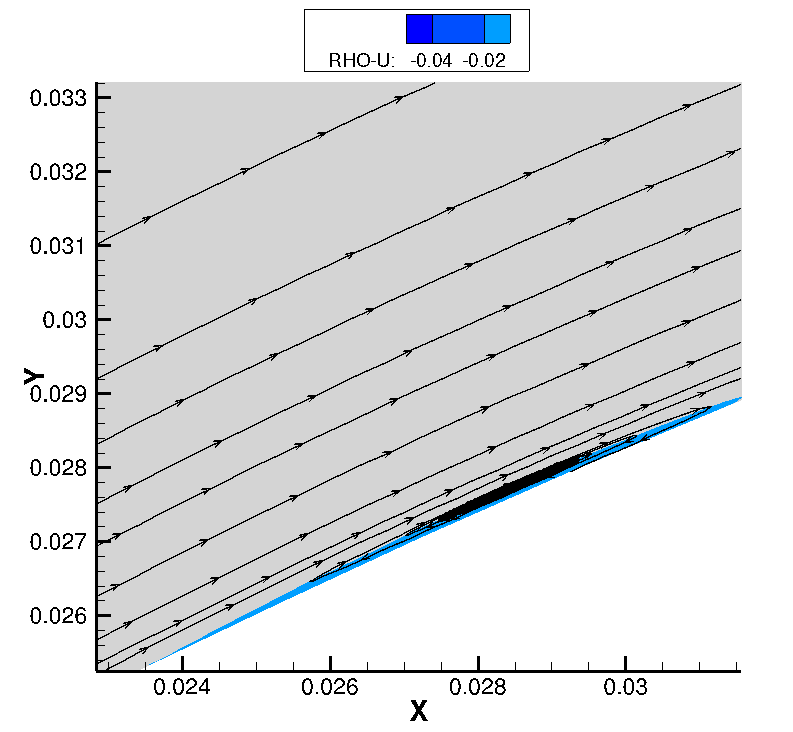
\includegraphics[width=1.0\textwidth]{./figs/recirculation_upper.png}
    \caption{Streamlines over the upper airfoil surface close to and inside the
        recirculation bubble. The blue region corresponds to the recirculation
        bubble.}\label{fig:recirculation_upper}
\end{figure}

\begin{figure}
    \centering
    \includegraphics[width=1.0\textwidth]{./figs/airfoil_sections.pdf}
    \caption{Various flow regimes over the airfoil. Profile locations are the locations
        at which u+ and y+ are plotted.}\label{fig:airfoil_sections}
\end{figure}





